\chapter{单纯空间与有向类型}
\section{同伦方向之外的单纯方向}
\begin{definition}[单纯空间]
单纯空间是一个函子
\[
C:\Delta^{\op}\longrightarrow\mathsf{Spaces}.
\]
为了使用已建立的模型，可将每个空间再表示为单纯集合，因而把 $C$ 写成双单纯集合 $C_{n,m}$。指标 $n$ 称为外单纯方向，指标 $m$ 称为内同伦方向。
\end{definition}
\begin{example}
固定外次数 $n$ 后，$m\mapsto C_{n,m}$ 表示一个空间 $C_n$。其中的路径与更高同伦由内方向编码。外方向的 $C_0,C_1,C_2$ 则分别将用于记录对象、箭头和三角形。这两种方向有不同的几何作用。
\end{example}
\begin{definition}[离散外形状]
若 $K$ 是单纯集合，将其每层集合视为离散空间，得到单纯空间，仍记作 $K$。特别地，$\Delta^n$、$\partial\Delta^n$、$\Lambda_k^n$ 和脊柱 $I[n]$ 都可以作为外形状。
\end{definition}
\begin{remark}
外形状 $\Delta^1$ 记录 $0\to1$。它的几何实现虽然是可缩区间，但在有向类型中不能因此把它等同于一个点。模型采用逐层弱等价；$\Delta^1$ 有两个外顶点，而一点只有一个，二者不是逐层等价。
\end{remark}
\begin{example}[两种不同的“路径”]
单纯空间 $C$ 的 $C_0$ 中的路径 $p:x=y$ 属于内同伦方向。一个外 $1$-单形 $f\in C_1$ 则具有源与靶 $x,y$。前者总能反向，后者未必能反向。后文用 $p:x=y$ 与 $f:x\to_Cy$ 分别表示它们。
\end{example}

\section{边界匹配对象}
\begin{definition}[匹配对象]
对单纯空间 $C$，$n$ 次匹配对象 $M_nC$ 由一个 $n$-单形的全部真面及其相容关系组成。形式上，它是所有单射 $[k]\hookrightarrow[n]$、$k<n$ 所给出的有限图表的极限。
\end{definition}
\begin{example}
低维情形为
\[
M_0C=\one,
\qquad M_1C=C_0\times C_0.
\]
$M_2C$ 的一点由三个对象和三条边组成，边的端点与这些对象相符。它记录三角形的边界，但尚未包含三角形内部的单形。
\end{example}
\begin{definition}[Reedy 纤维性]
称单纯空间 $C$ 为 Reedy 纤维的，若每个边界限制
\[
C_n\longrightarrow M_nC
\]
都是 Kan 纤维化。一个映射 $p:C\to D$ 为 Reedy 纤维化，若
\[
C_n\longrightarrow M_nC\times_{M_nD}D_n
\]
对所有 $n$ 都是 Kan 纤维化。
\end{definition}
\begin{proposition}
若 $C$ 为 Reedy 纤维的，则 $C_0$ 是 Kan 复形，且端点映射
\[
(d_1,d_0):C_1\to C_0\times C_0
\]
是 Kan 纤维化。因而其严格纤维表示所需的同伦映射空间。
\end{proposition}
\begin{proof}
分别取 $n=0,1$。$C_0\to\one$ 是 Kan 纤维化恰说明 $C_0$ 是 Kan 复形。端点映射的纤维由纤维化的拉回给出，因此也是 Kan 复形，并且计算同伦纤维。
\end{proof}
\begin{example}[离散单纯空间]
任意两个离散单纯集合之间的函数都是 Kan 纤维化。因为一个角及其填充单形到离散集合的映射都是常值，选定上方角的值后便唯一延拓。因此任意将每层看作离散空间的单纯集合都是 Reedy 纤维的。
\end{example}
\begin{remark}
把同一个 Kan 复形 $K$ 在外方向重复，并不一般给出 Reedy 纤维对象。它的 $1$ 次匹配映射是对角 $K\to K\times K$，而这一映射通常不是 Kan 纤维化。若需要把一个空间放入单纯空间模型，应使用合适的 Reedy 纤维替换或一个同伦常值的纤维模型。
\end{remark}

\section{单纯空间的模型结构}
\begin{theorem}[Reedy 模型结构，语义基础定理]
单纯空间具有 Reedy 模型结构：弱等价为逐层弱同伦等价，纤维化由上节的匹配映射条件给出，余纤维化为双单纯集合的单射。这个模型结构与内同伦方向的单纯富集相容。
\end{theorem}
\begin{remark}
这是 Reedy 模型结构在单纯集合上的具体应用。其证明沿次数递归，分别在每层使用边界的匹配对象与退化单形的闩锁对象，再应用单纯集合中的分解与提升。完整的一般定理见\cite{RiehlCatHomotopy,GoerssJardine}。本章以后使用该定理保证路径、依赖族和形状延拓在单纯参数中都有正确的纤维性。
\end{remark}
\begin{definition}[形状上的映射对象]
对有限外形状 $K$ 和单纯空间 $C$，以 $C^K$ 表示内部指数对象。它在外次数 $r$ 的空间为
\[
(C^K)_r=\Map_{\sSp}(\Delta^r\times K,C),
\]
其中右边的映射空间使用内同伦方向的富集。
\end{definition}
\begin{proposition}[带参数的形状图表]
从 $\Gamma$ 到 $C^K$ 的映射等价于从 $\Gamma\times K$ 到 $C$ 的映射。故 $C^K$ 记录所有参数中的 $K$ 形图表，而不只记录不带参数的图表。
\end{proposition}
\begin{proof}
这是指数对象的伴随关系。逐个内单纯次数应用预层范畴的指数公式，再检查外面映射与退化映射，得到自然双射。该双射随内单形变化，因而组成映射空间的同构。
\end{proof}
\begin{proposition}[限制映射的纤维性]
若 $C$ 为 Reedy 纤维的，$K\hookrightarrow L$ 为外形状的单射，则 $C^L\to C^K$ 是 Reedy 纤维化。
\end{proposition}
\begin{proof}
这是 Reedy 单纯模型结构的推积与指数相容性。把一个待解的提升图通过指数伴随转到 $C$ 一侧，左边成为形状单射与测试的平凡余纤维化的推积。该推积仍是平凡余纤维化，因而可对 $C\to\one$ 提升。再转回指数伴随即可。
\end{proof}

\section{同一性类型与有向同态类型}
\begin{definition}[有向同态类型]
对于有向类型 $C$ 中的 $x,y:C$，定义
\[
\Hom_C(x,y)=
\fib_{(\ev_0,\ev_1)}(x,y),
\qquad
C^{\Delta^1}\to C\times C.
\]
等价地，一个元素是函数 $f:\Delta^1\to C$，并固定端点 $f(0)=x$、$f(1)=y$。形状的边界条件在语法中可严格指定，在语义中由相应限制映射的纤维解释。
\end{definition}
\begin{definition}[恒等箭头]
常值形状函数 $\Delta^1\to C$ 给出 $\id_x:\Hom_C(x,x)$。
\end{definition}
\begin{proposition}[路径给出箭头]
有典范函数
\[
\mathsf{pathToArrow}:(x=y)\to\Hom_C(x,y),
\]
在常路径处取恒等箭头。
\end{proposition}
\begin{proof}
在族 $P(x,y,p)=\Hom_C(x,y)$ 中使用路径归纳，恒等情形给出 $\id_x$。此构造不需要预先假设 $C$ 有箭头合成。
\end{proof}
\begin{remark}
在任意有向类型中，一般没有从 $\Hom_C(x,y)$ 回到 $x=y$ 的函数。即使类型以后满足范畴公理，也只会将可逆箭头识别为路径。群胚条件则会进一步识别全部箭头与路径。
\end{remark}

\section{普通范畴的两种神经}
\begin{example}[离散神经]
对普通范畴 $\mathcal C$，其神经 $N\mathcal C$ 的每层作为离散空间，可看成单纯空间。其中 $C_0$ 是对象集合，$C_1$ 是态射集合，$C_n$ 是 $n$ 条可合成态射组成的链。箭头合成由普通合成给出。
\end{example}
\begin{remark}
如果 $\mathcal C$ 有两个不同但同构的对象，离散神经的对象空间内仍没有连接它们的路径。因此它可以满足合成条件，却不满足“对象路径恰好是对象同构”的完备性条件。
\end{remark}
\begin{definition}[分类图表]
对普通范畴 $\mathcal C$，令 $\mathcal C^\simeq$ 为保留全部对象和全部同构的群胚。定义单纯空间
\[
\mathsf{R}\mathcal C_n
=N\bigl(\Fun([n],\mathcal C)^\simeq\bigr).
\]
这里内方向的神经取在群胚上，外方向由预复合 $[k]\to[n]$ 给出。
\end{definition}
\begin{example}
$\mathsf{R}\mathcal C_0=N(\mathcal C^\simeq)$，所以对象之间的同构已成为对象空间中的路径。$\mathsf{R}\mathcal C_1$ 中，一个路径是两条态射间的可逆交换方形：
\[
\begin{tikzcd}
x\ar[r,"f"]\ar[d,"u"',"\cong"]&y\ar[d,"v","\cong"']\\
x'\ar[r,"f'"']&y'.
\end{tikzcd}
\]
交换条件为 $v\circ f=f'\circ u$。
\end{example}
\begin{remark}
分类图表连同所需的 Reedy 纤维模型，是将普通范畴放入完备 Segal 空间的标准方式。它保留对象的同构信息，而离散神经只在箭头层记录这些同构。二者的区别正是随后完备性条件要处理的内容\cite{Rezk}。
\end{remark}

\section{外部 Segal 映射}
\begin{definition}[脊柱]
$I[n]\subseteq\Delta^n$ 是由连续边
\[
0\to1\to\cdots\to n
\]
组成的子单纯集合。一个 $I[n]$ 形图表只指定 $n$ 条可合成箭头，不指定长边与较高单形。
\end{definition}
\begin{definition}[外部 Segal 条件]
Reedy 纤维单纯空间 $C$ 称为 Segal 空间，若对每个 $n\ge2$，映射
\[
C_n\longrightarrow
\underbrace{C_1\times_{C_0}\cdots\times_{C_0}C_1}_{n\text{ 个因子}}
\]
是空间的等价。由于端点映射为纤维化，所写拉回同时计算同伦拉回。
\end{definition}
\begin{example}
普通范畴的离散神经满足全部 Segal 条件，而且 Segal 映射是双射。因为一个函子 $[n]\to\mathcal C$ 由相邻边完全决定，所有长边都是相邻边的复合。
\end{example}
\begin{proposition}[只检验外部二次条件不足]
存在 Reedy 纤维单纯空间，其 $n=2$ 的外部 Segal 映射为等价，而 $n=3$ 的外部 Segal 映射不是等价。
\end{proposition}
\begin{proof}
将 $\partial\Delta^3$ 看作逐层离散的单纯空间。它与 $\Delta^3=N[3]$ 在 $0,1,2$ 次完全相同，因此 $n=2$ 的 Segal 映射为双射。链
\[
0\to1\to2\to3
\]
属于三重箭头拉回，却没有相应的非退化 $3$-单形，因为 $\partial\Delta^3$ 恰好删去了该内部单形。因此 $n=3$ 的映射不满射，不是等价。
\end{proof}
\begin{remark}
这个反例说明，后文 Riehl--Shulman 的内部二次条件不能读作这里只在外次数零检验的一条等价。内部条件要求指数对象间的等价，在每个参数语境中成立。这一更强的要求才足以控制全部较高合成。
\end{remark}

\section{单纯形的有向坐标}
\begin{definition}[有向区间与形状]
内部语言中用有向区间 $\Int$ 表示外 $\Delta^1$。在形状层允许次序关系与有限的交、并，由此写
\[
\Delta^n=\{(t_1,\ldots,t_n)\mid
1\ge t_1\ge\cdots\ge t_n\ge0\}.
\]
这些条件属于形状的边界语言，不等于断言每个内部类型都有一个这样的线性序。
\end{definition}
\begin{example}
$\Delta^2$ 的顶点为 $(0,0),(1,0),(1,1)$。内角 $\Lambda_1^2$ 是边 $t_2=0$ 与边 $t_1=1$ 的并。剩余边 $t_1=t_2$ 将表示复合箭头。
\[
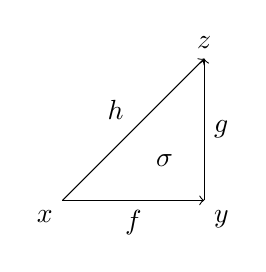
\begin{tikzpicture}[scale=1.8]
\draw[->] (0,0)--(1,0) node[midway,below]{$f$};
\draw[->] (1,0)--(1,1) node[midway,right]{$g$};
\draw[->] (0,0)--(1,1) node[midway,above left]{$h$};
\node[below left] at (0,0){$x$};\node[below right] at (1,0){$y$};\node[above] at (1,1){$z$};
\node at (.72,.28){$\sigma$};
\end{tikzpicture}
\]
三角形 $\sigma$ 将 $h$ 与先 $f$ 后 $g$ 的合成联系起来。
\end{example}
\begin{definition}[延拓类型]
对于形状包含 $K\hookrightarrow L$ 和边界图表 $a:K\to C$，延拓类型为
\[
\Ext_{K\subseteq L}(a)
=\fib_{C^L\to C^K}(a).
\]
其元素包含完整的 $L$ 形图表及与指定边界的相容。由于限制映射为纤维化，可在语法中把边界固定而无须每次重写等价的端点数据。
\end{definition}
\source{单纯空间语义与形状层的具体规则见\cite{RiehlShulman,RiehlICM}。本章先给出外部图表，再引入内部形状，以明确“所有语境中的等价”所包含的参数。
}
